\chapter{Background}

Thanks to a protective atmosphere, Earth can withstand impacts from dust-sized to boulder-sized objects traveling faster than bullets without so much as a dent on Earth's surface.
While most of these near-Earth objects are extremely small and don't leave much of a trace, the larger objects can leave a light trail visible from Earth's surface as they burn up in our atmosphere.
In this chapter, we will discuss the classification of near-Earth objects, the camera system and equations we will use for our analysis, the existing photometry tools we have, along with other existing surveys.


\section{Description of Fireballs}

When considering types of near-Earth objects, many names come to mind.  
Asteroids, meteors, meteorites, and fireballs are often used interchangeably. 
However, there are several key distinctions between these objects.  
Asteroids are the largest of this group and are generally over $10$m in diameter \cite{meteoroidorbits}. 
These large objects are responsible for large craters that are visibly present on the moon.  
Meteoroids are anywhere between $10 \mu$m and $10$m and are drastically more common than asteroids.  

Meteoroids that pass through earth's atmosphere become meteors.
As meteors pass through the atmosphere, they begin to ablate, or release light.  
This phenomena happens because the interactions between the meteor molecules with the air molecules produce lots of energy, some of which goes into the production of light.
This light can be measured in terms of apparent magnitude.
Magnitude is represented on a $\log_10$ scale and dimmer objects are represented by high numbers while brighter objects are lower.  
If the meteor releases visible light below an apparent magnitude of $-4$ qualify as bolides, or fireballs.
For reference, Venus is a magnitude $-4.4$ planet while the dimmer Jupiter has a magnitude of $-2.1$.


If an object is massive enough to withstand the pressures of Earth's atmosphere and make it to the surface of Earth, it is classified as a meteorite. 
These are extremely uncommon, but provide valuable information about the rock's origin.
Figure \ref{jed} shows the relationship between these 4 objects.

\begin{figure}[ht!]
  \centering
  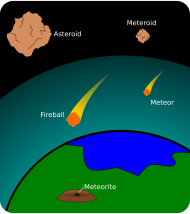
\includegraphics[scale=0.5]{images/jedmasterpiece.png}
  \caption{A depiction of near-Earth object classification.}
  \label{jed}
\end{figure}

We may further classify near-Earth objects into two categories: sporadic events and meteor shower events. 
Meteor showers occur when Earth's orbit crosses paths with the orbit of a collection of debris. 
Such collections often orbit large masses such as Jupiter or the sun \cite{trigo-rodriguez_2006_2007}.  
For example, the Perseid meteor shower has a highly elliptical orbit around the sun as seen in Fig. \ref{perceid}.  
A majority of the composition of these showers stems from the decomposition of comets throughout space.  

\begin{figure}[ht!]
  \centering
  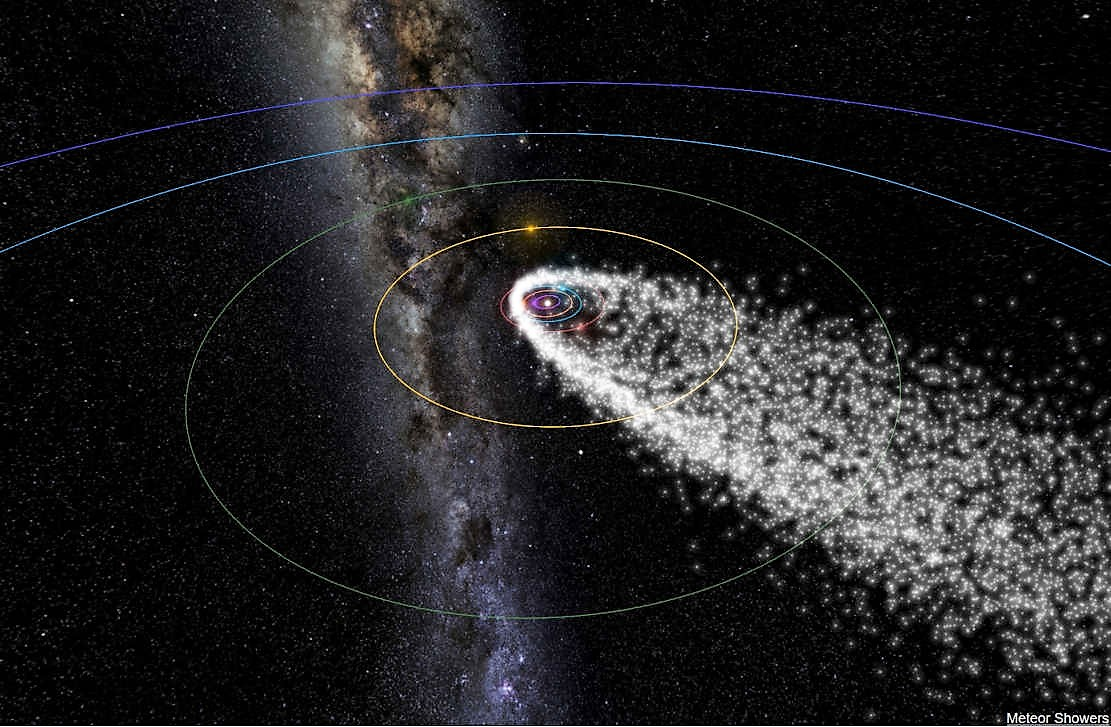
\includegraphics[scale=0.7]{images/persiod_shower.jpg}
  \caption{The Perseid meteor shower and its relation to our solar system.}
  \label{perceid}
\end{figure}

In contrast, there is debris in space that is not connected to any meteor shower. 
These are called sporadic events. 
Because gravity tends to bring objects together, we see mostly collections of debris.
However, when objects escape their collection due to other interactions (gravitational or electromagnetic), they still have a chance of colliding with Earth.

Studying these near-Earth objects can give us good estimates for how many objects you might expect to see pass through a given area of space within a specific amount of time. 
This measurement is called flux.
By determining flux, we can more accurately predict the 


\section{The D6 AllSky Camera}

\subsection{Composition}



\subsection{Uniqueness}







\section{Photometry}

\subsection{Existing photometry tools}



\subsection{Airplanes and other interference}







\section{Analysis}

\subsubsection{Parameters of Interest}



\subsection{Flux}







\section{Existing Surveys}
While amateur astronomers and low-budget systems capture useful information, larger professional systems act as a vitally important comparison point.
Individual events captured by an observer do contribute to the pursuit of knowledge.
However, a small camera system that cannot yield similar data to more professional surveys serves only a marginal amount of utility.
Cameras for AllSky Meteor Surveillance (CAMS), the SPanish Meteor Network (SPMN), and the Lincoln Near Earth Asteroid Research (LINEAR) program are examples of well-established existing meteor observing surveys.  
All of these programs are continuously acquiring data and adding their findings to existing databases.  
Nearly all of this data is widely available, and is available to the public online. 



\subsection{CAMS}
Funded by NASA, Cameras for Allsky Meteor Surveillance (CAMS) aims to verify minor meteor showers and trace them back to their existing parent comets \cite{jenniskens_cams:_2011}.  
The project was created by Peter Jenniskens and is based in California.  
The CAMS network is spread across 3 different locations and consists of over 60 cameras.
Each camera is has a relatively narrow field of view $~30\deg$.
Although they individually cover a small area, multiple cameras overlapping in field of view contribute to a large sky coverage. 
CAMS uses powerful CCD cameras to detect extremely dim meteors (up to around $+5$ mag).
By spreading their cameras across three separate locations, the CAMS research group can measure extremely precise trajectories of the incoming meteors. 
Similarly to the phenomena of trying to catch a baseball with only one eye open, confidently capturing a three dimensional trajectory of a fireball is extremely difficult when using only one camera.
Consisting of $3$ cameras located within $25$ miles of one another, as seen in Fig. \ref{trio} the CAMS survey have a median trajectory error of $0.31\deg$ and a median speed error of $0.53$ km/s \cite{jenniskens_cams:_2011}. 

\begin{figure}[ht!]
  \centering
  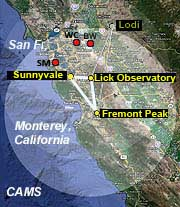
\includegraphics[scale=0.7]{images/CAMS_trio.jpg}
%   \setcaptioncitation{http://cams.seti.org/maps.html}
  \caption{The three CAMS network stations within a $50$ mile radius.}
  \label{trio}
\end{figure}

Accurate trajectories are particularly useful in back-tracing the motion of the meteor's orbit.  
The CAMS team has reduced over $320,000$ of these orbits \cite{seticams}. 
In addition to calculating orbits, CAMS also uses their precise velocity measurements to draw relations between speed and other properties. 
Figure \ref{fancyCAMS} shows the relationship between the apparent incident speed and peak magnitude.

\begin{figure}[ht!]
  \centering
  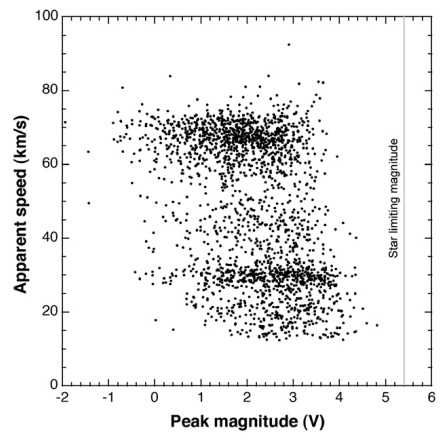
\includegraphics[scale=0.6]{images/CAMS_plot.png}
  \caption{Relationship between incident apparent speed and peak magnitude for CAMS data taken in November of 2010 \cite{jenniskens_cams:_2011}.}
  \label{fancyCAMS}
\end{figure}


Although the plot itself doesn't show a linear relationship, when considering the two subsets of relatively higher and lower incident speeds, we can see a general trend.
That trend shows that lower incident speed meteors tend to have slightly dimmer peak magnitudes. 



\subsection{SPMN}

The SPanish Meteor Network (SPMN) works extremely similarly to the CAMS project.  
It consists of $25$ observation stations located across Portugal and Spain \cite{trigo-rodriguez_2006_2007}.
Figure \ref{SPan} shows the approximate coverage of these stations along with some proposed locations (in green), from a satellite point of view.  

\begin{figure}[ht!]
  \centering
  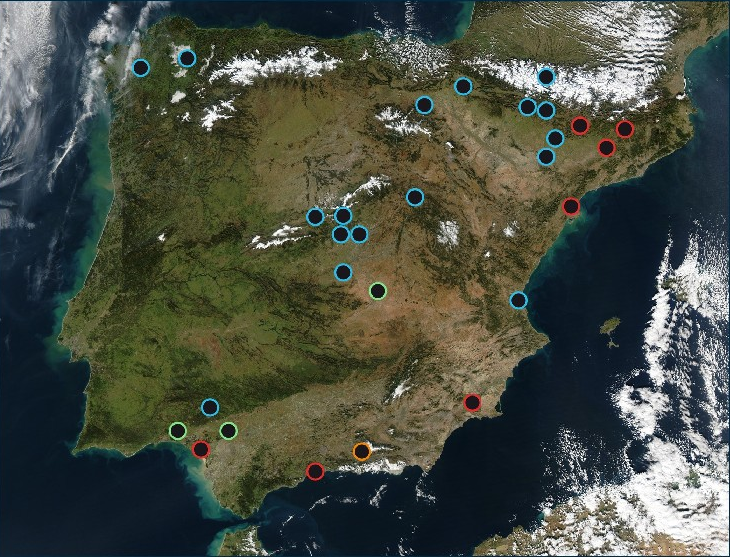
\includegraphics[scale=0.3]{images/satalite_of_love.png}
  \caption{Satellite view of the SPanish Meteor Network's sky coverage across $25$ existing and $3$ proposed observation stations  \cite{Spanish}.}
  \label{SPan}
\end{figure}

In addition to becoming the first organization in Spain to successfully calculate the orbital path of a meteor, this organization revolutionized fireball research by developing the first CCD AllSky cameras \cite{Spanish}.
These cameras are now in use all across the world.
While the SPMN and CAMS are extremely powerful research organizations, their study of meteors only slightly overlaps with the research being discussed in this paper.
Because of their high grade equipment, they are able to capture data from extremely dim sources.
Fireballs, quantified by a magnitude below $-4$, compose only a small fraction of the meteors analyzed by these organizations.
Fortunately, other organizations focus specifically on larger and brighter events.

\subsection{Other research groups}

There are a multitude of ways that one can attain information about a fireball.  
All the aforementioned surveys have employed the use of photometric data.
Peter Brown, a well renowned fireball researcher, took data from the Department of Defense and the Department of Energy space-based systems in geostationary orbits.
The original purpose of these systems is to detect signatures of explosions near earth's surface, but occasionally pick up false positives in the form of bolides.  
Because the systems detect the amount of power released, scientists such as Peter Brown can approximate the fireball's energy.
In a 2002 article published by \textit{Nature}, Brown estimated the optical energies of around 300 bolides.
From this data set and other existing data sets, Brown created Eq. \ref{browneq}, which relates bolide energy to the number of impacts on earth each year. 

\begin{figure}[ht!]
  \centering
  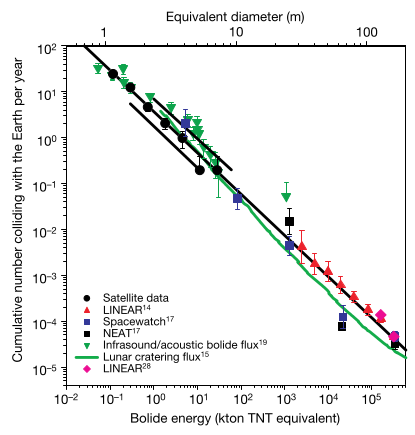
\includegraphics[scale=0.7]{images/flux_brown.png}
  \caption{A plot of bolide flux using an conglomeration of data \cite{brown_p_flux_2002}.}
  \label{powerlaw}
\end{figure}


Figure \ref{powerlaw} shows this relationship alongside data taken from many different research groups.  

In his research, Brown used existing assumptions (mentioned in the Analysis section) for the blackbody distribution and the velocity.  



